\documentclass{scrartcl}
\usepackage[utf8]{inputenc}
\usepackage[english]{babel} % Trennung nach der neuen deutschen Rechtschreibung
\usepackage[utf8]{inputenc}
\usepackage[T1]{fontenc}
\usepackage{lmodern}

\usepackage{amsmath} % Erweiterte Mathematik-Umgebung
\usepackage{amsfonts} % zusätzliche Mathematik-Schrifttypen (v.a. \mathbb für Mengen)
\usepackage{ulem}

\usepackage{graphics}%soll beim Graphiken einfügen hilfreich sein
\usepackage{graphicx}
\usepackage{wrapfig}%lässt Textumflossene Bildeinbindung zu
\usepackage{epstopdf}%soll eps in pdf umwandeln

\usepackage[a4paper, portrait, margin=2.5cm]{geometry}

\titlehead{\centering University of Luxemburg}
\subject{Travaux Pratiques}
\title{Adiabatic coefficients}
\subtitle{Alberto Garilli}
\date{TP Session 29/10/2021}
\author{Louis-Hendrik Barboutie \\ Frederik Ehl \\ Florence Schmerber}

\begin{document}

\maketitle

\clearpage

\tableofcontents
\listoffigures
	
\clearpage

\section{Introduction}
In today's experiment, we want to calculate the adiabatic coefficients of four different gases. The adiabatic coefficient is the ratio of the heat capacity at constant pressure $C_P$ to heat capacity at constant volume $C_V$. We can consider our experiment to be adiabatic, which means there is no heat entering or leaving the system.
In order to determine the adiabatic coefficient $\gamma$, we will be measuring the frequency of oscillation using a cylinder with a movable piston, filled with gas.

\subsection{Experimental setup}
This experiment consist of a gas law apparatus (1). By pushing the piston down, we compress the gas inside the cylinder which results into a change of pressure. The apparatus is connected to a pressure sensor (2), which will then send the data to a special program, where it is plotted in a graph.
\begin{figure}[h]
    \centering
    \includegraphics[width=10cm]{IMG_20211101_103850.jpg}
    \caption{Experimental setup}
    \label{fig:my_label}
\end{figure}

\section{Adiabatic Coefficients}

\subsection{Procedure}

For this experiment we want to construct a graph that depicts the initial starting height $h$ of the piston as a function of the oscillation period. For that we repeat the same procedure for our 4 different gases.
First we fill the piston with the gas of our choice.The movable piston of area $A=\pi \cdot r^2$ and mass $m_p$ of a cylinder, filled with gas to a certain height $h$, is set in motion by pushing down and there by deflected from its equilibrium. The pressure differences are measured by the program Pascocapstone. We are interested in the oscillation of the piston when we put pressure on it and release it, because the gas will act like a spring and oscillate for a short period around the equilibrium point. The program plots this and for precision we measure the time of several periods, which we then divide by the amount of periods in that time frame to get one period $T$. We do that for different initial heights $h$.
We plot the height $h$ as a function of the period squared $T^2$. Then we plot the linear fit and write down the slope.
With this slope $s$ we can easily calculate the adiabatic coefficient with the relation:
\begin{equation}
\gamma=\frac{s4\pi^2 m}{pA}
\end{equation}
With $m$ being the weight of the piston (35,0g), $p$ the atmospheric pressure ($p=101,325kPa$) and $A$ the cross-sectional area of the piston ($A\approx8,2958\cdot10^{-4}m^2$).
we repeat that same procedure for all gases.

\subsection{Results}

\subsubsection{Air}
For Air we obtained the following values:

\medskip
\centering
\begin{tabular}{|c|c|}
    \hline
     $h  \ (10^{-3}m) $& $T  \ (s)$  \\
     \hline
     $95$ & $0,03675$ \\
     \hline
     $74$ & $0,033$ \\
     \hline
     $49$ & $0,029$ \\
     \hline
     $40$ & $0,026$ \\
     \hline
     $25$ & $0,022$ \\
     \hline
\end{tabular}
\flushleft
By plotting the function $h(T^2)$ and applying the linear fit we get a slope $s\approx81,5576$. We can now calculate the adiabatic coefficient of air using equation (1). We find \boxed{$\gamma_{air}\approx1,34$}

\subsubsection{CO_2}
For $CO_2$ we find the following values:

\medskip
\centering
\begin{tabular}{|c|c|}
    \hline
     $h  \ (10^{-3}m) $& $T  \ (s)$  \\
     \hline
     $91$ & $0,03725$ \\
     \hline
     $73$ & $0,03333$ \\
     \hline
     $55$ & $0,03$ \\
     \hline
     $35$ & $0,0254$ \\
     \hline
\end{tabular}
\flushleft
For $CO_2$ the slope $s$ of the function $h(T^2)$ is $\approx75,9850$, which results in \boxed{$\gamma_{CO_2}\approx1,25$}

\subsubsection{Helium}
For Helium we obtain 

\medskip
\centering
\begin{tabular}{|c|c|}
    \hline
     $h  \ (10^{-3}m) $& $T  \ (s)$  \\
     \hline
     $93$ & $0,03433$ \\
     \hline
     $82$ & $0,03375$ \\
     \hline
     $69$ & $0,03025$ \\
     \hline
     $55$ & $0,028$ \\
     \hline
     $40$ & $0,0246$ \\
     \hline
     $27$ & $0,02175$ \\
     \hline
     $17$ & $0,0193$ \\
     \hline
\end{tabular}
\flushleft
\textbf{Remark:} Here we choose to ignore the first two measurements. In fact, the density of helium is less than the density of air, therefore it "floats on top" of the remaining air in the cylinder. Since we evacuate gases through the bottom of the cylinder, it is mainly air we are flushing out of the system when lowering the piston. Therefore the lower the initial height, the higher the ratio of helium to air, and the more accurate our computations of $\gamma$ become.

For the slope of the function $h(T^2)$ for Helium we find $s\approx94,4492$. So we obtain \boxed{$\gamma_{He}\approx1,55$.}

\subsubsection{Nitrogen}
Our measurements for Nitrogen gave the following results

\medskip

\centering
\begin{tabular}{|c|c|}
    \hline
     $h  \ (10^{-3}m) $& $T  \ (s)$  \\
     \hline
     $93$ & $0,03567$ \\
     \hline
     $73$ & $0,033$ \\
     \hline
     $58$ & $0,0296$ \\
     \hline
     $41$ & $0,0271$ \\
     \hline
\end{tabular}
\flushleft
This time we calculate the slope of the function $h(T^2)$ to be $s\approx93,4193$ and therefore \boxed{$\gamma_{N_2}\approx1,535$}

\subsection{Comparison}

\centering
\begin{tabular}{|c|c|c|c|}
    \hline
    $gas$ & $\gamma_{experimental}$ & $\gamma_{Literature}$ & $deviation$ \\
    \hline
    $Air$ & $1,35$ & $1,40$ & $4,28\%$ \\
    \hline
    $Carbon \ Dioxide$ & $1,25$ & $1,29$ & $3.10\%$ \\
    \hline
    $Helium$ & $1,47$ & $1,63$ & $4,71\%$ \\
    \hline
    $Nitrogen$ & $1,535$ & $1,40$ & $8,79\%$ \\
    \hline
\end{tabular}
\flushleft

\section{Conclusion}
During this experiment we were able to determine the adiabatic coefficients of different gases. We obtained very satisfying values for Air and $CO_2$, whereas the one for Nitrogen deviated quite a bit. 

However we encountered problems with the measurement device: it produced a very noisy graph, which made it more difficult to accurately determine the periods, especially for Nitrogen. Furthermore we weren't given the purity of the gases, and we couldn't maintain a 100\% purity inside our system, which further lead to errors.

\section{Appendix}

\begin{figure}[h]
    \centering
    \includegraphics[width=12cm]{Graph_air.eps}
    \caption{Air}
    \label{fig:my_label}
\end{figure}

\begin{figure}
    \centering
    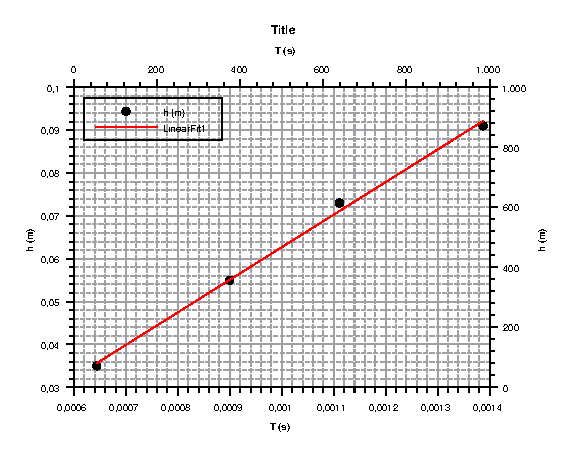
\includegraphics[width=12cm]{Graph_CO2.eps}
    \caption{$CO_2$}
    \label{fig:my_label}
\end{figure}

\begin{figure}
    \centering
    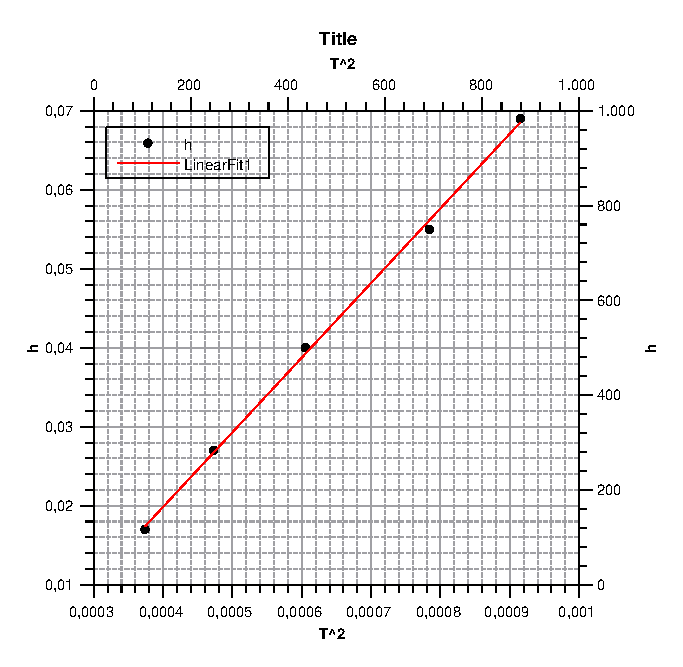
\includegraphics{Graph7.eps}
    \caption{Helium}
    \label{fig:my_label}
\end{figure}

\begin{figure}[h]
    \centering
    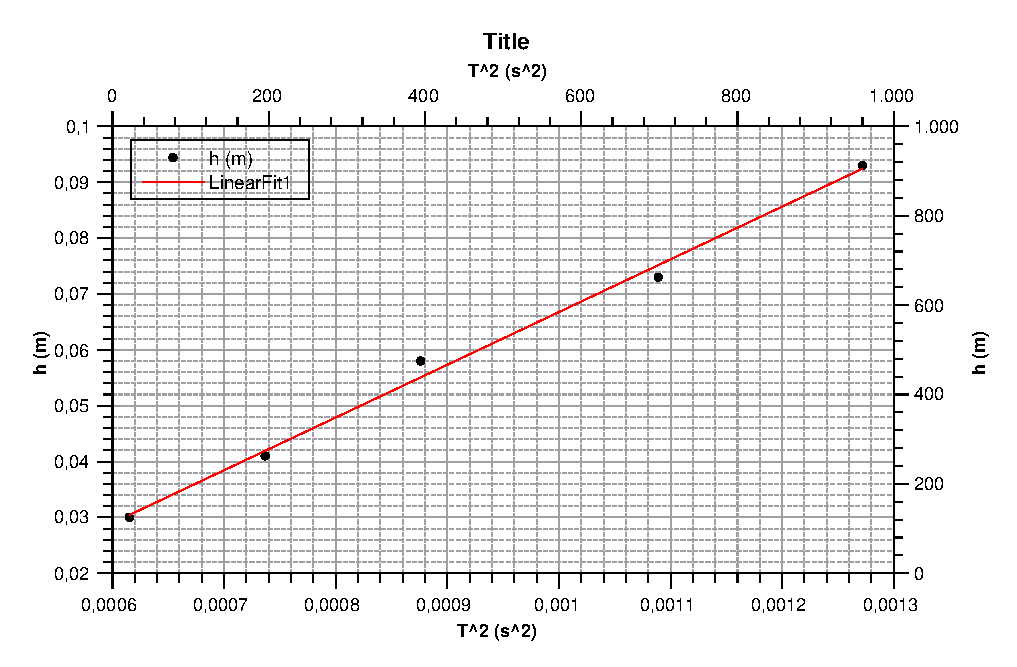
\includegraphics[width=12cm]{Graph5.eps}
    \caption{Nitrogen}
    \label{fig:my_label}
\end{figure}

\end{document}